\section{Results}
This chapter presents the results of the exploratory data analysis conducted across the three data sources: the Baumkataster, the Sentinel-2 satellite imagery, and the OpenStreetMap urban context layers, as well as the extended analysis of two additional training cities, Innsbruck and Linz. The goals of the analysis were to assess data quality, validate feature distributions, and identify the indicators most likely to be informative for the U-Net model.

\subsection{Baumkataster Analysis}
\subsubsection{Dataset Overview and Tree Density}

The cleaned Baumkataster data contain 226{,}998 trees for Vienna, 217{,}454 for Paris, 233{,}505 for Hamburg, and 43{,}367 for Barcelona. Comparing these raw counts directly is misleading because the bounding boxes scraped for each city differ substantially in area. Normalising by the official administrative area of each city (Figure~\ref{fig:tree-density}) yields a more informative comparison: Paris registers approximately 2{,}063 trees per km² of city area, far exceeding the other three cities, while Hamburg, whose scraped bounding box covers nearly 4{,}000~km², has the lowest density at 309 trees per km².

\begin{figure}[h]
\centering
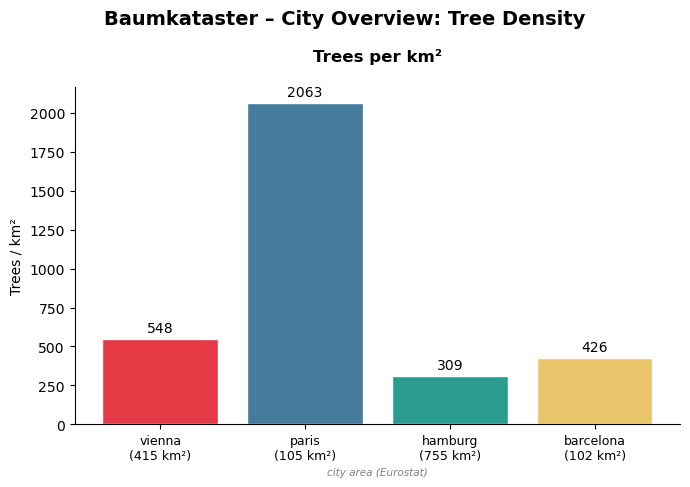
\includegraphics[width=0.6\textwidth]{images/eda_p2_fig01.png}
\caption{Tree density per km² of administrative area per city.}
\label{fig:tree-density}
\end{figure}

\subsubsection{Label Reliability: Temporal Misalignment, Private Property, and Removed Trees}
Three systematic biases in the cadastre labels are relevant to any modelling interpretation of performance metrics.

\textbf{Temporal misalignment.}
The Baumkataster datasets are snapshots rather than continuously updated registers. Vienna and Hamburg are updated roughly annually; the Paris dataset was last substantially revised around 2023; the Barcelona dataset dates from approximately 2017--2019. The Sentinel-2 composites used in this project are 2025 median mosaics, placing the cadastre labels two to six years behind the imagery. A tree planted after the last cadastre update that is already visible in 2025 will carry no positive label; a tree that has since been removed will retain one. Both cases inject noise into the supervision signal and set a practical ceiling on the model's achievable recall and precision when measured against the cadastre.

\textbf{Private-property trees.}
Municipal cadastres register only publicly owned or publicly accessible trees. Trees on private land, such as courtyard trees, garden trees, trees on institutional grounds are almost entirely absent. Barcelona is the most extreme case, partly explaining its comparatively low count despite a per-km² density otherwise comparable to Vienna. For the model this creates a systematic false-negative pressure during training: the satellite detects green NDVI signal from unregistered private canopy, but those pixels carry no positive label and are treated as background. The task should therefore be framed as detecting \emph{canopy} rather than detecting \emph{registered trees}, with precision and recall measured against the cadastre as an operationally useful proxy rather than a complete ground truth.

\textbf{Removed trees.}
The inverse problem: a cadastre entry surviving after a tree has been felled or died introduces a complementary false-positive pressure. The NDVI signal at that location resembles built or bare surface, but the label is positive. This effect is geographically scattered and smaller in magnitude than the private-property gap, but it cannot be resolved without a cadastre snapshot contemporaneous with the imagery.

\subsubsection{Vienna Data Corrections}
Two encoding issues specific to Vienna were identified and corrected before any further analysis. First, the \texttt{height} column stores ordinal category codes~0--8 representing height intervals from $<$5~m to $>$35~m, not continuous metres. Second, the \texttt{crown\_diameter} column uses the same ordinal scheme linked to crown-diameter intervals. Both were decoded to interval midpoints (Table~\ref{tab:vienna-decode}). Additionally, 415 Vienna circumference values of zero were found to encode unknown measurements and were replaced with NaN.

\begin{table}[h]
\centering
\caption{Vienna ordinal code decoding scheme applied to \texttt{height} and
\texttt{crown\_diameter}.}
\label{tab:vienna-decode}
\begin{tabular}{ccccc}
\hline
\textbf{Code} & \textbf{Height class} & \textbf{Midpoint (m)} &
\textbf{Crown class} & \textbf{Midpoint (m)} \\
\hline
0 & nicht bekannt & NaN   & nicht bekannt & NaN  \\
1 & 0--5~m        & 2.5   & 0--3~m        & 1.5  \\
2 & 6--10~m       & 8.0   & 4--6~m        & 5.0  \\
3 & 11--15~m      & 13.0  & 7--9~m        & 8.0  \\
4 & 16--20~m      & 18.0  & 10--12~m      & 11.0 \\
5 & 21--25~m      & 23.0  & 13--15~m      & 14.0 \\
6 & 26--30~m      & 28.0  & 16--18~m      & 17.0 \\
7 & 31--35~m      & 33.0  & 19--21~m      & 20.0 \\
8 & $>$35~m       & 37.5  & $>$21~m       & 22.5 \\
\hline
\end{tabular}
\end{table}

After decoding, the Vienna height distribution has a median of~8.0~m and a mean of~8.9~m, closely matching Paris (median 8.0~m, mean 9.0~m), validating the decoding scheme against an independent source. The corrected Hamburg trunk circumference mean (121.6~cm) exceeds Vienna (98.0~cm) and Paris (82.3~cm), consistent with Hamburg's dominance by large-crowned \textit{Quercus robur} and \textit{Tilia~$\times$~europaea}. Figures~\ref{fig:size-dist}--\ref{fig:size-dist-f} shows the corrected size distributions across cities.

\begin{figure}[htbp]
\centering
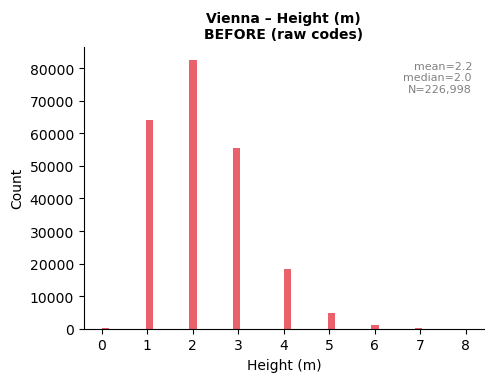
\includegraphics[width=0.7\textwidth, height=0.38\textheight,keepaspectratio]{images/eda_p2_fig04_a.png}
\caption{Vienna --- tree height, before correction (raw ordinal codes).}
\label{fig:size-dist}
\end{figure}

\begin{figure}[htbp]
\centering
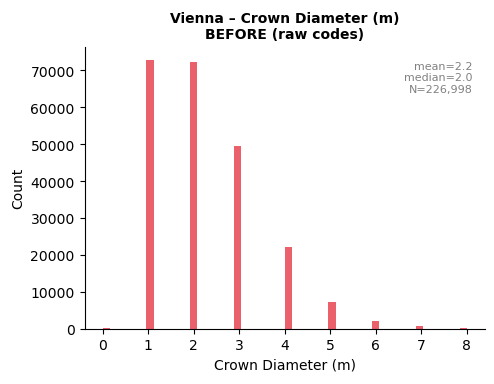
\includegraphics[width=0.7\textwidth, height=0.38\textheight,keepaspectratio]{images/eda_p2_fig04_c.png}
\caption{Vienna --- crown diameter, before correction (raw codes).}
\label{fig:size-dist-c}
\end{figure}

\begin{figure}[htbp]
\centering
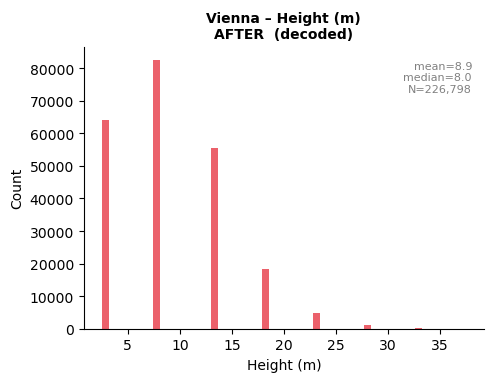
\includegraphics[width=0.7\textwidth,height=0.38\textheight,keepaspectratio]{images/eda_p2_fig04_d.png}
\caption{Vienna --- tree height, after correction (decoded to metres).}
\label{fig:size-dist-d}
\end{figure}

\begin{figure}[htbp]
\centering
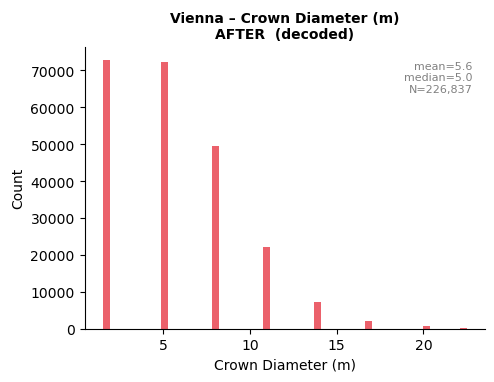
\includegraphics[width=0.7\textwidth, height=0.38\textheight,keepaspectratio]{images/eda_p2_fig04_f.png}
\caption{Vienna --- crown diameter, after correction (decoded to metres).}
\label{fig:size-dist-f}
\end{figure}

\clearpage
\subsubsection{Species Composition}

Species diversity is high across all cities: 670 unique species in Vienna, 996 in Paris, 354 in Hamburg, and 330 in Barcelona, with 86 species shared across all four cities, predominantly from the \textit{Abies} and \textit{Acer} genera. Vienna is dominated by \textit{Acer platanoides} (Norway maple, 19{,}244 trees) and \textit{Aesculus hippocastanum} (horse chestnut, 11{,}661 trees), both classic central-European street species. Paris is dominated by \textit{Platanus~$\times$~hispanica} (London plane, 38{,}113~trees). Hamburg is dominated by \textit{Quercus robur} (English oak, 42{,}965~trees) and \textit{Tilia~$\times$~europaea} (European lime, 33{,}852~trees). Barcelona shows a distinct Mediterranean composition including subtropical species such as \textit{Tipuana tipu} and \textit{Pinus pinea}. Species identity is not a direct model input, but species diversity informs expectations about canopy shape and size variation across cities.

\subsubsection{Spatial Distribution and Label Imbalance}
Figures~\ref{fig:spatial-scatter}--\ref{fig:spatial-scatter-c} shows that tree locations are distributed unevenly within each city. Raw patch sampling would therefore oversample dense clusters and underrepresent sparser districts, potentially producing a model that performs well on dense parkland but fails on isolated street trees. The patch-sampling strategy must account for this imbalance, for instance through stratified sampling or spatially weighted loss functions.

\begin{figure}[htbp]
\centering
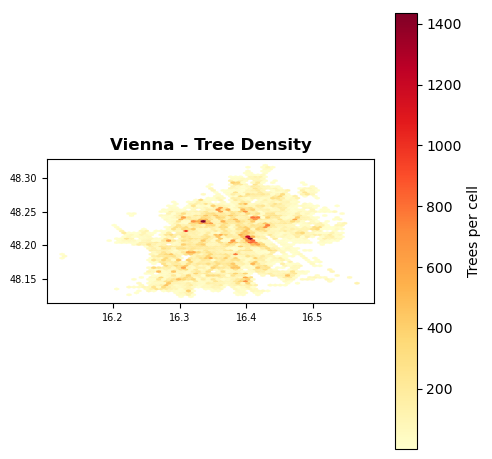
\includegraphics[width=0.8\textwidth, height=0.38\textheight,keepaspectratio]{images/eda_fig06_a.png}
\caption{Vienna. Spatial distribution of labelled tree locations.}
\label{fig:spatial-scatter}
\end{figure}

\begin{figure}[htbp]
\centering
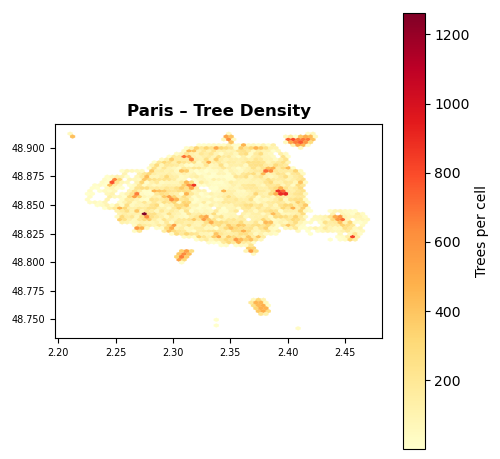
\includegraphics[width=0.8\textwidth, height=0.38\textheight,keepaspectratio]{images/eda_fig06_b.png}
\caption{Paris.}
\label{fig:spatial-scatter-b}
\end{figure}

\begin{figure}[htbp]
\centering
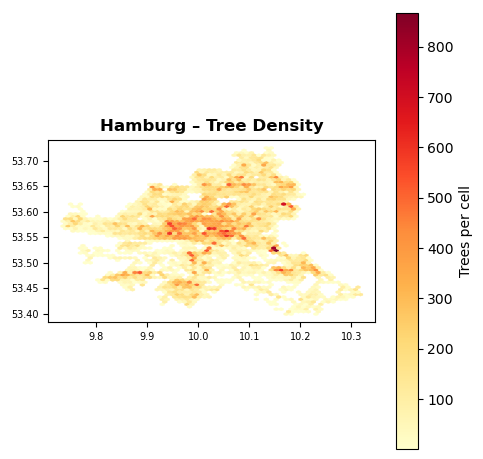
\includegraphics[width=0.8\textwidth, height=0.38\textheight,keepaspectratio]{images/eda_fig06_c.png}
\caption{Hamburg.}
\label{fig:spatial-scatter-c}
\end{figure}

\newpage
\subsection{Sentinel-2 Analysis}
\label{sec:results-sentinel}

All 12 city-season Sentinel-2 composites (four cities $\times$ three seasons) were successfully loaded and validated. The seven available channels are B02 (blue), B03 (green), B04 (red), B08 (NIR), NDVI, EVI, and SAVI.

\subsubsection{EVI and SAVI Scaling Correction}
A systematic quality issue was identified: EVI and SAVI were computed from raw Sentinel-2 digital number (DN) values in the range $\approx 0$--$10{,}000$ rather than from surface-reflectance values in $[0, 1]$. Because both formulas contain an additive constant in the denominator (EVI: $+1$; SAVI: $+0.5$), this constant is overwhelmed when band values are on the order of $10^{3}$, causing EVI to substantially exceed its theoretical bound of $+1.0$. NDVI is unaffected because it is a pure ratio and is therefore scale-invariant.

The correction was applied by dividing all raw band values by $10{,}000$ before recomputing EVI and SAVI. After correction, EVI values lie within $[-1, 1]$ across all cities and seasons (Figures~\ref{fig:evi-savi}--\ref{fig:evi-savi-d}), confirming the fix. Corrected TIF stacks were saved to \texttt{data\_after\_eda/sentinel~data/}.

\begin{figure}[htbp]
\centering
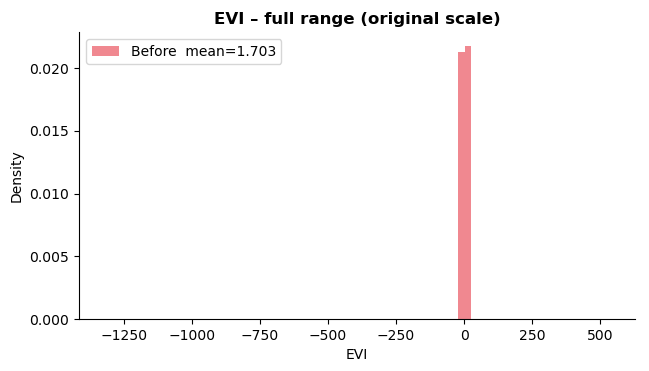
\includegraphics[width=0.72\textwidth, height=0.38\textheight,keepaspectratio]{images/eda_p2_fig09_a.png}
\caption{EVI --- full range (original scale).}
\label{fig:evi-savi}
\end{figure}

\begin{figure}[htbp]
\centering
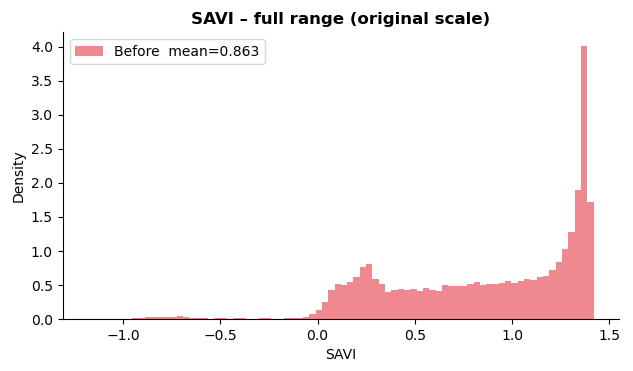
\includegraphics[width=0.72\textwidth, height=0.38\textheight,keepaspectratio]{images/eda_p2_fig09_b.png}
\caption{SAVI --- full range (original scale).}
\label{fig:evi-savi-b}
\end{figure}

\begin{figure}[htbp]
\centering
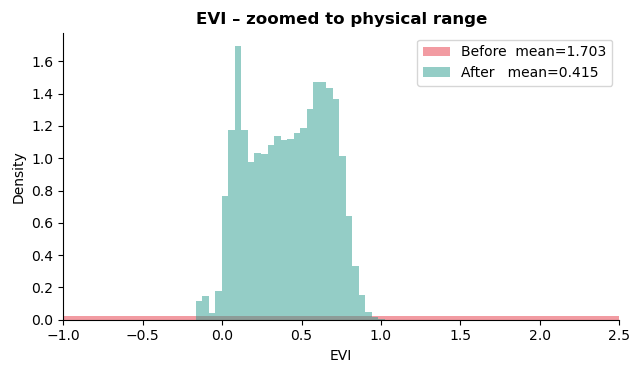
\includegraphics[width=0.72\textwidth, height=0.38\textheight,keepaspectratio]{images/eda_p2_fig09_c.png}
\caption{EVI --- zoomed to the physical range.}
\label{fig:evi-savi-c}
\end{figure}

\begin{figure}[htbp]
\centering
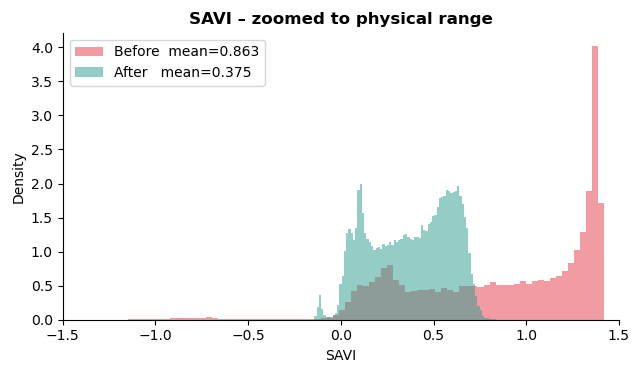
\includegraphics[width=0.72\textwidth, height=0.38\textheight,keepaspectratio]{images/eda_p2_fig09_d.png}
\caption{SAVI --- zoomed to the physical range.}
\label{fig:evi-savi-d}
\end{figure}

\subsubsection{NDVI Seasonal Patterns}
Table~\ref{tab:ndvi} shows mean NDVI values per city and season. The seasonal pattern is city-specific rather than uniform, and the visual summary is shown in Figure~\ref{fig:ndvi-seasonal}.

\begin{table}[h]
\centering
\caption{Mean NDVI by city and season. The Paris autumn value corresponds to October
imagery, as no November composite was available.}
\label{tab:ndvi}
\begin{tabular}{lrrr}
\hline
\textbf{City} & \textbf{Spring (Apr)} & \textbf{Summer (Aug)} & \textbf{Autumn (Oct/Nov)} \\
\hline
Vienna    & 0.563 & 0.577 & 0.457 \\
Paris     & 0.371 & 0.396 & 0.476 \\
Hamburg   & 0.295 & 0.418 & 0.347 \\
Barcelona & 0.281 & 0.287 & 0.287 \\
\hline
\end{tabular}
\end{table}

Vienna and Hamburg show their highest NDVI in summer (0.577 and 0.418 respectively), consistent with temperate deciduous canopies reaching full leaf-out in August. Barcelona is near-flat across all three seasons (0.281--0.287), reflecting its Mediterranean, evergreen-dominated species composition and mild seasonal amplitude. Paris is the notable exception: its autumn NDVI (0.476) exceeds both its spring (0.371) and summer (0.396) values, an anomaly that requires a contextual explanation.

\begin{figure}[h]
\centering
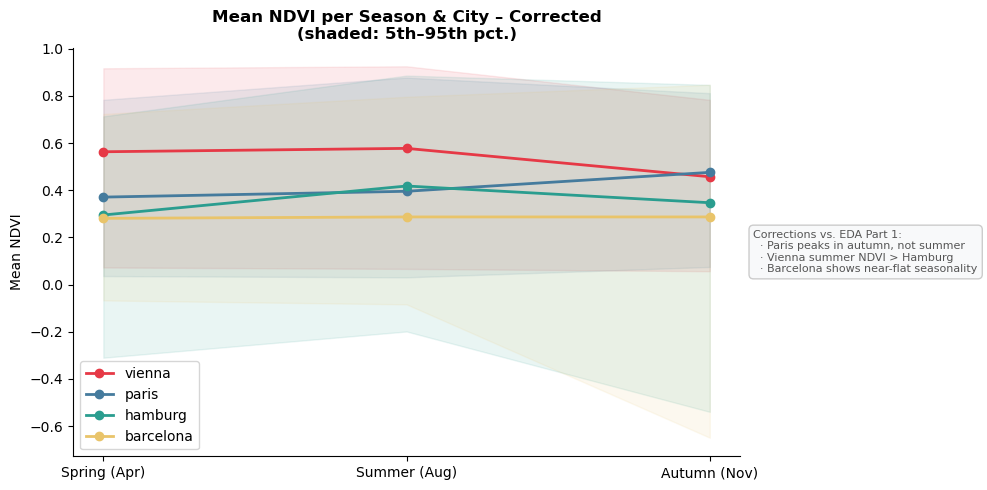
\includegraphics[width=0.75\textwidth, height=0.38\textheight,keepaspectratio]{images/eda_p2_fig08.png}
\caption{Mean NDVI per season and city.}
\label{fig:ndvi-seasonal}
\end{figure}

\newpage
\subsubsection{Paris NDVI and the 2024 Olympics Urban Reforestation}
The Paris autumn NDVI value (0.476) exceeds both its spring (0.371) and summer (0.396) means, inverting the temperate-deciduous pattern seen in Vienna and Hamburg. It is tempting to read this as a signature of the city's large-scale greening programme: under a 2020 commitment, Paris set out to plant 170{,}000 trees between 2020 and 2026, with roughly 8{,}900 of them concentrated in and around the Olympic Village in Seine-Saint-Denis for the 2024 Summer Games (The Local, 2020; Monocle, 2026). Because the Sentinel-2 composites used here are 2025 mosaics, they postdate both the Games and much of this effort.

On closer inspection, however, attributing the autumn peak to reforestation is difficult to defend. First, the planting is poorly matched to what a coarse vegetation index can resolve. Only about 63{,}500 of the 170{,}000 target had been planted by mid-2023 (Euronews Green, 2023), so a large share of the trees visible to the 2025 imagery are one to three growing seasons old; newly planted street trees have crowns far smaller than the 10~m Sentinel-2 pixel and contribute negligibly to pixel-level NDVI in their first years. Second, a single city-wide seasonal mean is too aggregate an instrument to isolate a spatially concentrated intervention: even if the Seine-Saint-Denis plantings raised NDVI locally, that signal would be diluted across the full administrative area and would not preferentially inflate the \emph{autumn} value relative to summer.

A simpler explanation is already present in the data. As noted in Table~\ref{tab:ndvi}, the Paris ``autumn'' composite is built from October imagery because no cloud-free November mosaic was available, whereas the other cities use November. October in Paris falls before full leaf senescence, so a green October composite sits systematically above a true late-autumn one. The apparent autumn~$>$~summer inversion is therefore most parsimoniously a compositing artefact rather than a phenological or anthropogenic one. A depressed August value under summer heat or drought stress could compound the effect, but this cannot be confirmed from the present data and is not asserted here.

This reframing matters for how the reforestation enters the project. The seasonal NDVI curve is derived from reflectance and is independent of the Baumkataster, so the planting programme does not ``explain'' the NDVI anomaly. Its concrete consequence is instead one of label quality: the Paris cadastre was last substantially revised around 2023 and predates most Olympic-era planting, so the 2025 imagery contains canopy, particularly in the northern arrondissements, that carries no positive label. Paris is therefore the city with the most severe label-to-image temporal misalignment in the corpus, and evaluation metrics computed over Parisian patches in these districts should be read with that undercount in mind.

\subsubsection{False-Color Composites}
Figure~\ref{fig:false-color} shows false-color composites (NIR~$\to$~red, red~$\to$~green, green~$\to$~blue) for all four cities across all three seasons, rendered from corrected TIF stacks.In this encoding, healthy vegetation appears bright red, built surfaces grey-cyan, and
water near-black. The composites confirm that the Sentinel-2 data are correctly georeferenced and that vegetation is clearly separable from urban surfaces across all cities and seasons. Seasonal changes in canopy density are visible for Vienna and Hamburg between summer and autumn. Barcelona's canopy remains consistent across all three composites with its near-flat NDVI.

\begin{figure}[h]
\centering
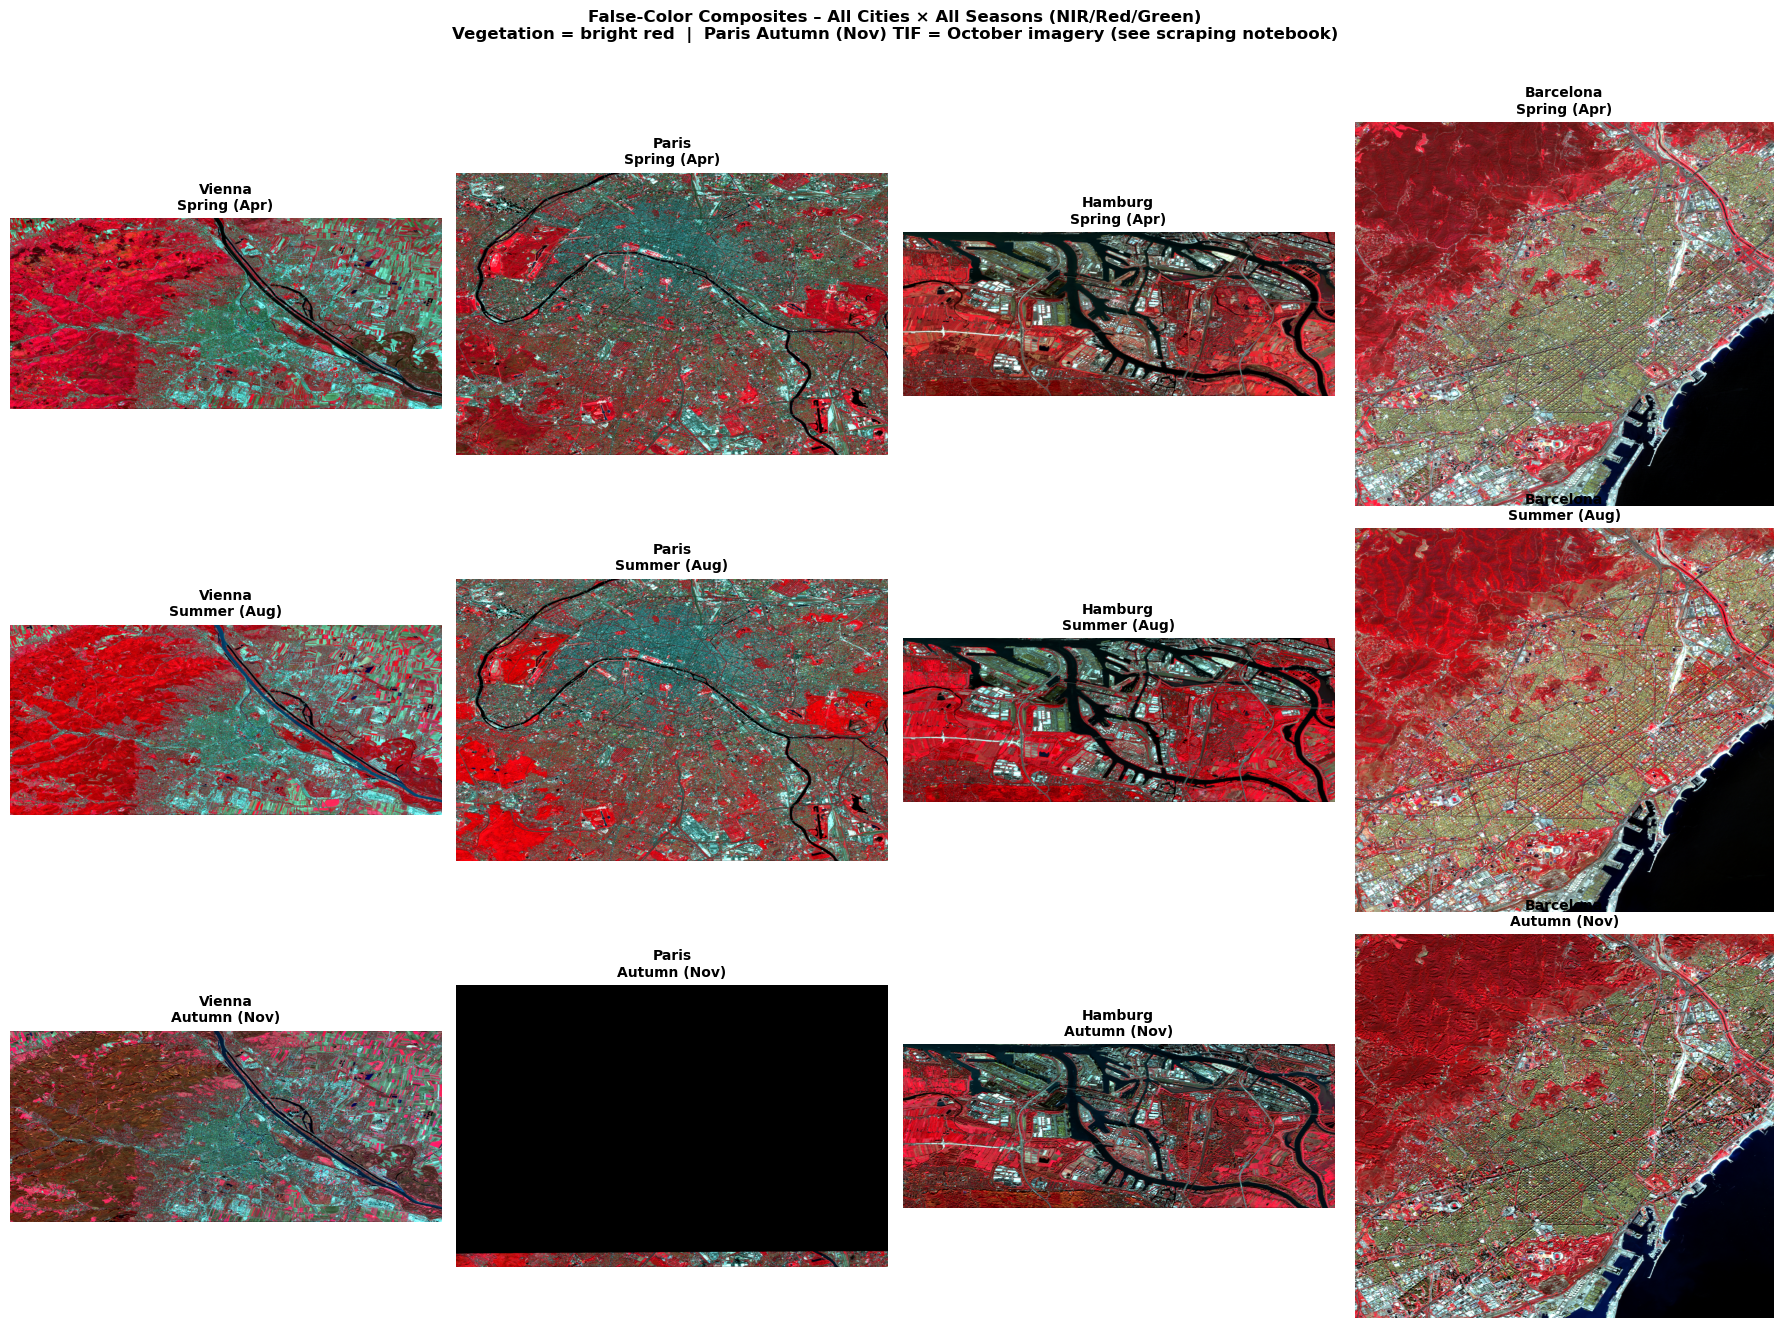
\includegraphics[width=\textwidth]{images/eda_p2_fig10.png}
\caption{False-color composites (NIR/Red/Green) for all four cities.}
\label{fig:false-color}
\end{figure}

\newpage
\subsection{OSM Analysis}
\subsubsection{OSM as a Community Project: Cross-City Coverage and Semantic Consistency}
OpenStreetMap is a volunteer-contributed dataset, and its coverage and the \emph{semantics} of its tags vary significantly across cities.
This has direct consequences for any analysis that treats OSM labels as ground truth for vegetation or land cover.

\textbf{Vienna} benefits from one of the most active national OSM communities in Europe. The Austrian contributor base maintains fine-grained \texttt{park}, \texttt{forest}, and \texttt{grass} tags that are generally reliable and up to date.

\textbf{Hamburg} presents a documented gap: the road network is densely mapped (161{,}378 features), but the landuse layer is substantially sparser than expected given the city's comparable tree-cadastre count, with only 24{,}184 road features in the
landuse extract. This reflects genuine mapping gaps in residential green space rather than a scraping or clipping issue.

\textbf{Paris} has strong OSM coverage in the central arrondissements but patchy coverage in the outer banlieues. Critically, the Seine-Saint-Denis districts that received the bulk of the Olympic-era tree plantings are likely under-mapped in the landuse layer, compounding the label-temporal-misalignment problem discussed in Section~\ref{sec:results-paris-olympics}.

\textbf{Barcelona} has reasonable OSM coverage for public parks and major green zones, but private green space---which is substantial given Barcelona's dense, enclosed \textit{illa} block structure---is almost never tagged.

Beyond coverage gaps, a deeper semantic problem exists: the tags \texttt{park}, \texttt{garden}, \texttt{grass}, and \texttt{forest} do not encode equivalent vegetation densities across cities. A Viennese \textit{Stadtpark} is a formal, heavily tree-canopied park with high NDVI;
a \texttt{park} tag in Barcelona may refer to a small, partly paved plaza with a few ornamental trees. Treating these as a binary green/not-green mask in the cross-dataset analysis of Section~\ref{sec:results-tree-counts} conflates very different vegetation structures. For model training, OSM landuse is therefore best used as a \emph{contextual covariate} that provides spatial priors about likely versus unlikely tree locations, not as ground truth for vegetation presence.

\subsubsection{Road Type Distribution}
Figures~\ref{fig:road-type} shows the road-type composition per city. Footway, service, and residential classes dominate in Barcelona, Paris, and Vienna. Hamburg is the exception, where service roads outnumber footways. Only wider classes (primary, secondary, motorway) are suitable as reliable tree-free negative-label candidates for mask generation. Narrower classes such as path, steps, and track frequently run through parks alongside trees and must not be used as hard negative masks.

\begin{figure}[htbp]
\centering
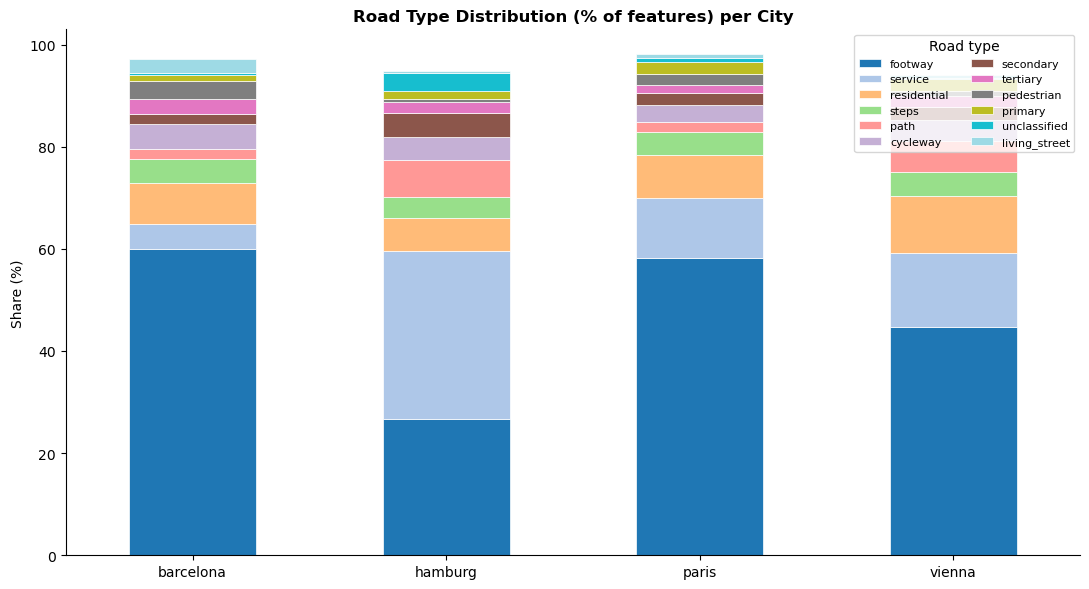
\includegraphics[width=0.82\textwidth, height=0.38\textheight,keepaspectratio]{images/eda_fig_rt.png}
\caption{Road-type distribution per city as a percentage of total road features.}
\label{fig:road-type}
\end{figure}

\newpage
\subsubsection{Land Use Distribution}
Figures~\ref{fig:landuse}--\ref{fig:landuse-d} shows the land use distribution by area. Vienna and Paris contain large mapped green-area polygons; Hamburg's landuse layer is notably sparser, consistent with the mapping gap described above. Building footprints are spatially reliable for all four cities and will be used as hard negative-label zones during training mask generation, since no trees are expected
on rooftop surfaces.

\begin{figure}[htbp]
\centering
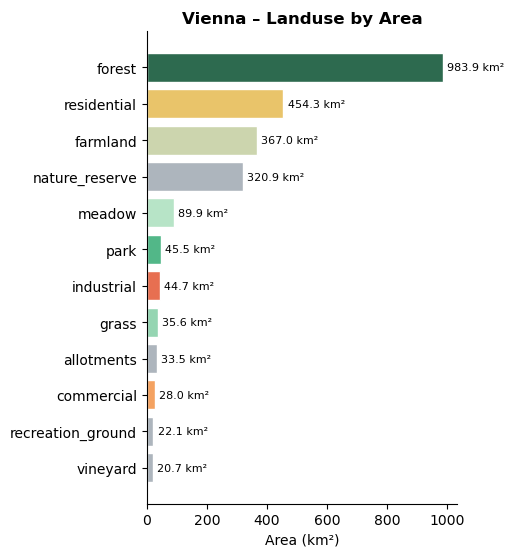
\includegraphics[width=0.72\textwidth, height=0.38\textheight,keepaspectratio]{images/eda_fig12_a.png}
\caption{Land use distribution by area per city. Vienna.}
\label{fig:landuse}
\end{figure}

\begin{figure}[htbp]
\centering
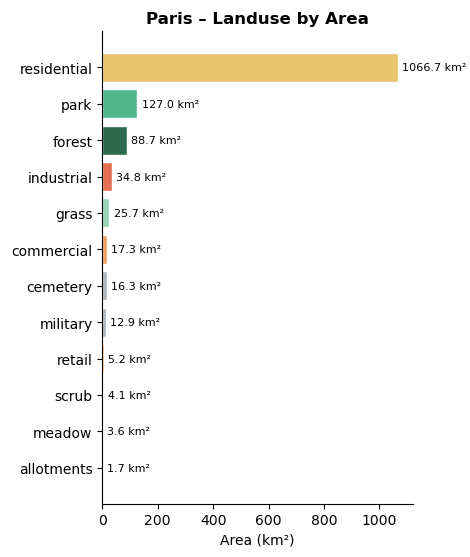
\includegraphics[width=0.72\textwidth, height=0.38\textheight,keepaspectratio]{images/eda_fig12_b.png}
\caption{Paris.}
\label{fig:landuse-b}
\end{figure}

\begin{figure}[htbp]
\centering
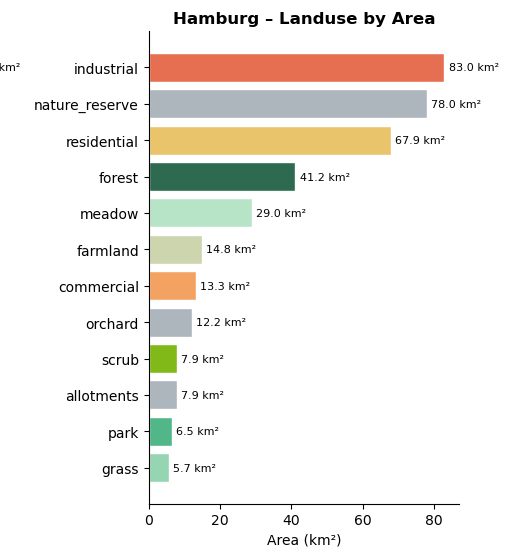
\includegraphics[width=0.72\textwidth, height=0.38\textheight,keepaspectratio]{images/eda_fig12_c.png}
\caption{Hamburg.}
\label{fig:landuse-c}
\end{figure}

\begin{figure}[htbp]
\centering
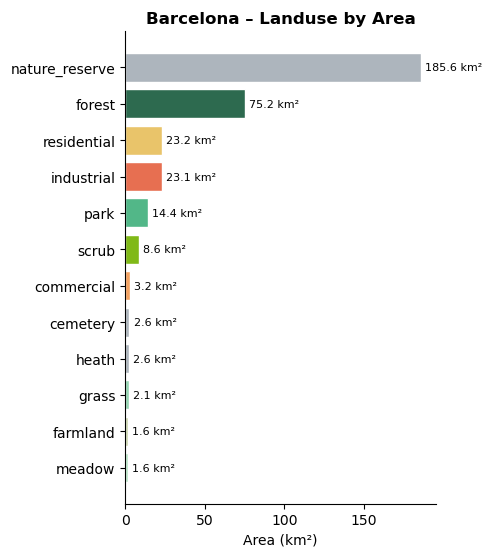
\includegraphics[width=0.72\textwidth, height=0.38\textheight,keepaspectratio]{images/eda_fig12_d.png}
\caption{Barcelona.}
\label{fig:landuse-d}
\end{figure}

\newpage
\subsection{Extended Training Corpus: Innsbruck and Linz}
Two additional Austrian cities, Innsbruck and Linz, were added to expand the training
corpus with urban environments of different morphological character and with a stronger
Austrian context for generalisation testing.

\subsubsection{Baumkataster: Innsbruck and Linz}

The Innsbruck Baumkataster contains 13{,}656 trees described by longitude, latitude,
species, and city identifier only; no morphological attributes are available.
Linz provides a richer dataset of 26{,}866 trees including continuous height (m), crown
diameter (m), circumference (cm), and a binary \texttt{type\_of\_tree} flag
distinguishing deciduous (\texttt{L}, 24{,}053 trees, 89.5\%) from coniferous
(\texttt{N}, 2{,}813 trees, 10.5\%).
Table~\ref{tab:new-cities} summarises the two datasets.

\begin{table}[h]
\centering
\caption{Short summary for the Innsbruck and Linz Baumkataster datasets.}
\label{tab:new-cities}
\begin{tabular}{lrrll}
\hline
\textbf{City} & \textbf{Trees} & \textbf{Species} & \textbf{Top species} \\
\hline
Innsbruck & 13{,}656 & 304 & \textit{A.\ platanoides} (5.4\%) \\
Linz      & 26{,}866 & 374 & \textit{A.\ platanoides} (7.0\%) \\
\hline
\end{tabular}
\end{table}

Species diversity is consistent with the primary training cities, and the dominant
species across both---\textit{Acer platanoides} (Norway maple)---is also the leading
species in Vienna, Hamburg, and Barcelona, confirming a coherent central-European
temperate flora.
117 species are shared between Innsbruck and Linz (20.9\% of the combined union of
561 species).
Figures~\ref{fig:species-innsbruck-linz}--\ref{fig:species-innsbruck-linz-b} shows the species distributions for both cities.

\begin{figure}[htbp]
\centering
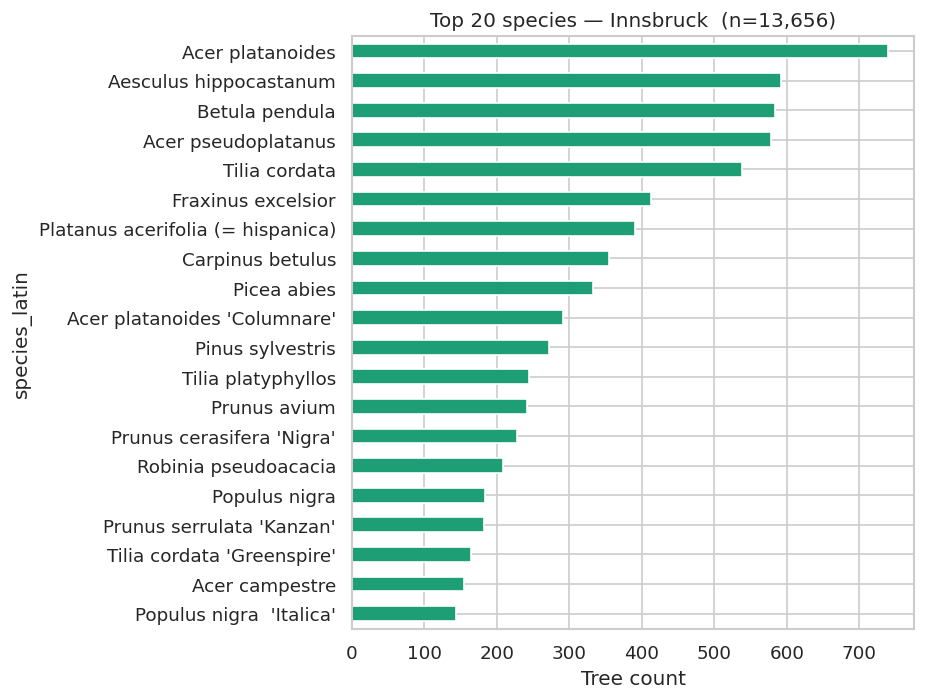
\includegraphics[width=0.62\textwidth]{images/eda_p3_fig01_a.png}
\caption{Innsbruck. Species distribution and long-tail analysis for Innsbruck and Linz. A small number of species accounts for the majority of trees, with \textit{Acer platanoides} dominant in both cities.}
\label{fig:species-innsbruck-linz}
\end{figure}

\begin{figure}[htbp]
\centering
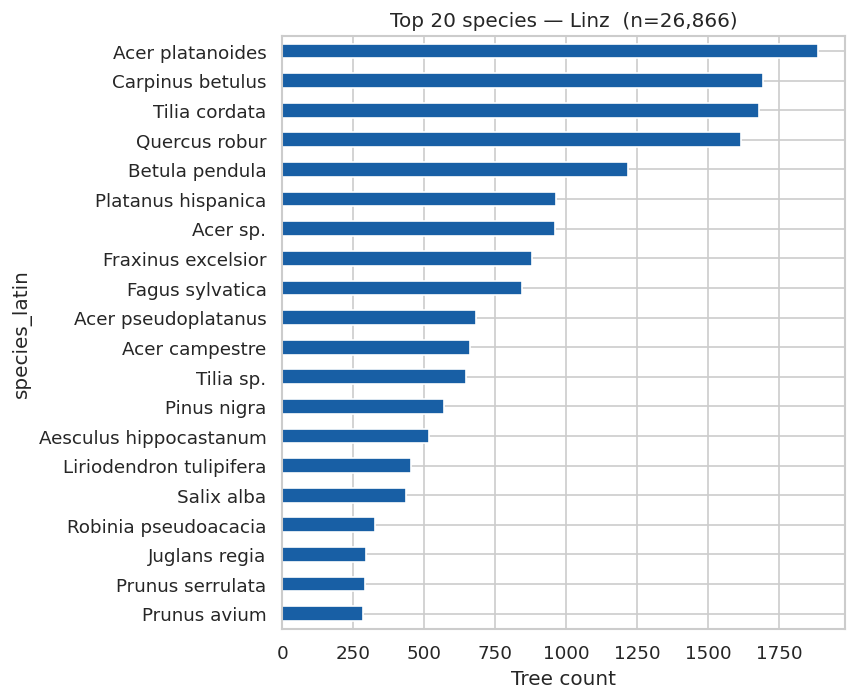
\includegraphics[width=0.62\textwidth]{images/eda_p3_fig01_b.png}
\caption{Linz.}
\label{fig:species-innsbruck-linz-b}
\end{figure}

\newpage
\subsubsection{Morphological Features and Data Quality: Linz}

Figures~\ref{fig:linz-morphology} shows the distributions of height and circumference for Linz, together with species-level boxplots.
The distributions are realistic and follow expected biological ranges for urban trees
in a temperate climate.

\begin{figure}[htbp]
\centering
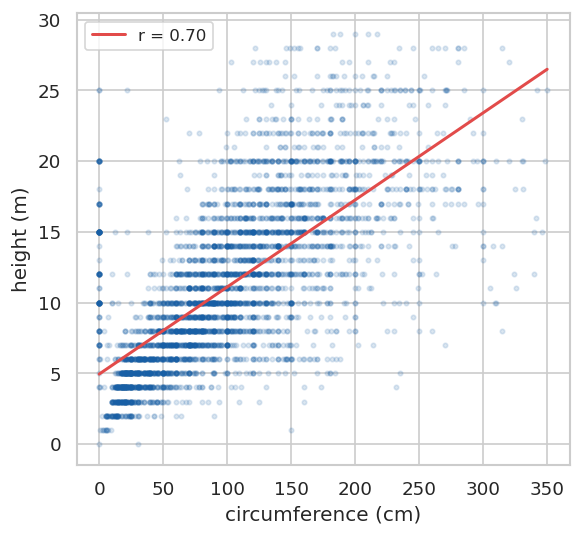
\includegraphics[width=0.7\textwidth]{images/eda_p3_fig05_a.png}
\caption{Trunk circumference vs.\ height. Morphological feature distributions for Linz.}
\label{fig:linz-morphology}
\end{figure}

IQR-based outlier inspection identifies a small number of likely data-entry errors at
the top 0.1\% of each column: one \textit{Fagus sylvatica} record lists a height of
151~m (physically impossible; probable unit confusion) and one \textit{Salix alba}
record lists a circumference of 11{,}120~cm (likely entered in millimetres rather than
centimetres).
These records should be capped or excluded before model training.

Coniferous trees have a higher median height (13.0~m vs.\ 10.0~m for deciduous) and
larger trunk circumference (110~cm vs.\ 90~cm), while deciduous trees have slightly
wider crowns.
These biologically plausible patterns validate data quality and suggest that the
\texttt{type\_of\_tree} flag could serve as a useful auxiliary label if the model is
extended to species-type classification.

\newpage
\subsubsection{Spatial Distribution: Innsbruck and Linz}

Figure~\ref{fig:linz_dens}--\ref{fig:ins_dens} shows the spatial distribution of trees in Innsbruck and
Linz.
Both cities exhibit the characteristic non-uniform clustering seen in the primary
training cities: trees are concentrated in boulevard networks and larger parks, with
sparser coverage in industrial and newer residential zones.
The combined corpus overview (Figures~\ref{fig:geospatial-new}--\ref{fig:combined-corpus-b}) confirms that adding
Innsbruck and Linz increases the total labelled tree count by 40{,}522 trees and extends
the geographic and morphological range of the training data.

\begin{figure}[htbp]
\centering
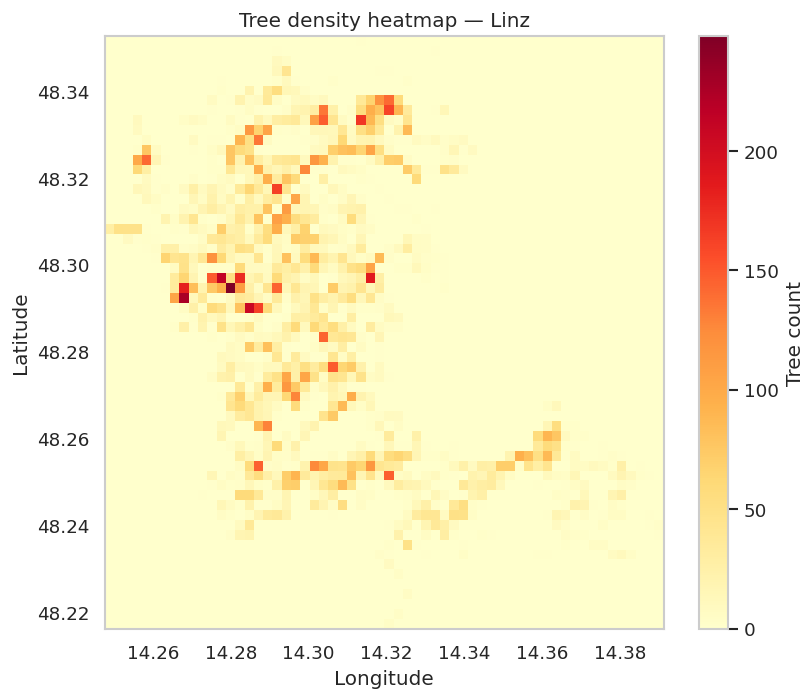
\includegraphics[width=0.74\textwidth]{images/eda_p3_fig09_a.png}
\caption{Tree density heatmap. Linz.}
\label{fig:linz_dens}
\end{figure}

\begin{figure}[htbp]
\centering
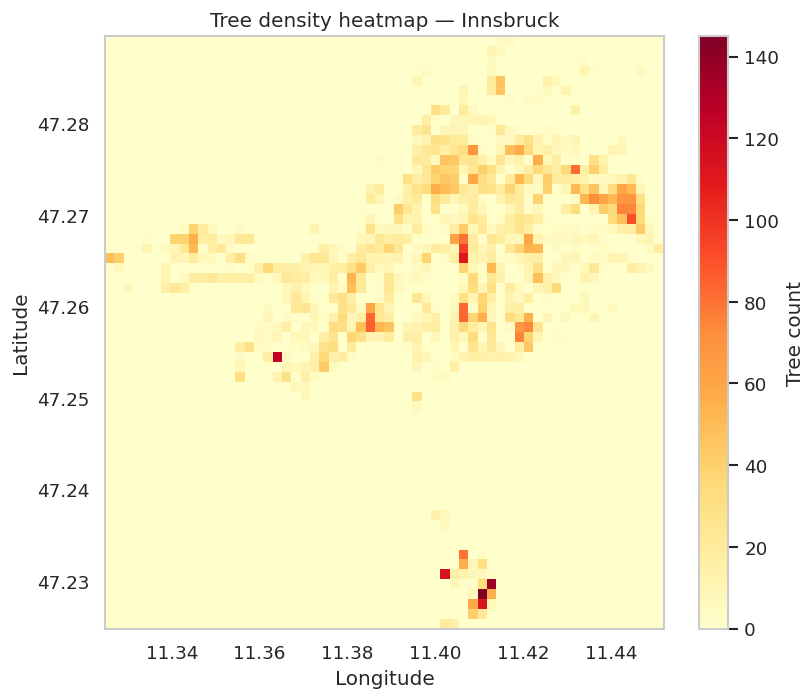
\includegraphics[width=0.74\textwidth]{images/eda_p3_fig09_b.png}
\caption{Innsbruck.}
\label{fig:ins_dens}
\end{figure}

\newpage
\subsubsection{OSM: Innsbruck and Linz}

OSM data for both cities were loaded across roads, buildings, landuse, and water layers.
Linz has 57{,}702 road features and 62{,}006 building footprints; Innsbruck has 22{,}064
and 24{,}337 respectively, proportional to their populations.
Figure~\ref{fig:osm-new} shows the feature-class distributions.
Both cities benefit from active Austrian OSM contributor communities and show comparably
complete coverage to Vienna.
Building footprints are spatially reliable for negative-label masking.
The same cross-city semantic caveats about green-space tag interpretation apply, although
the risk is lower in the Austrian context where OSM norms are more consistent.

\begin{figure}[h]
\centering
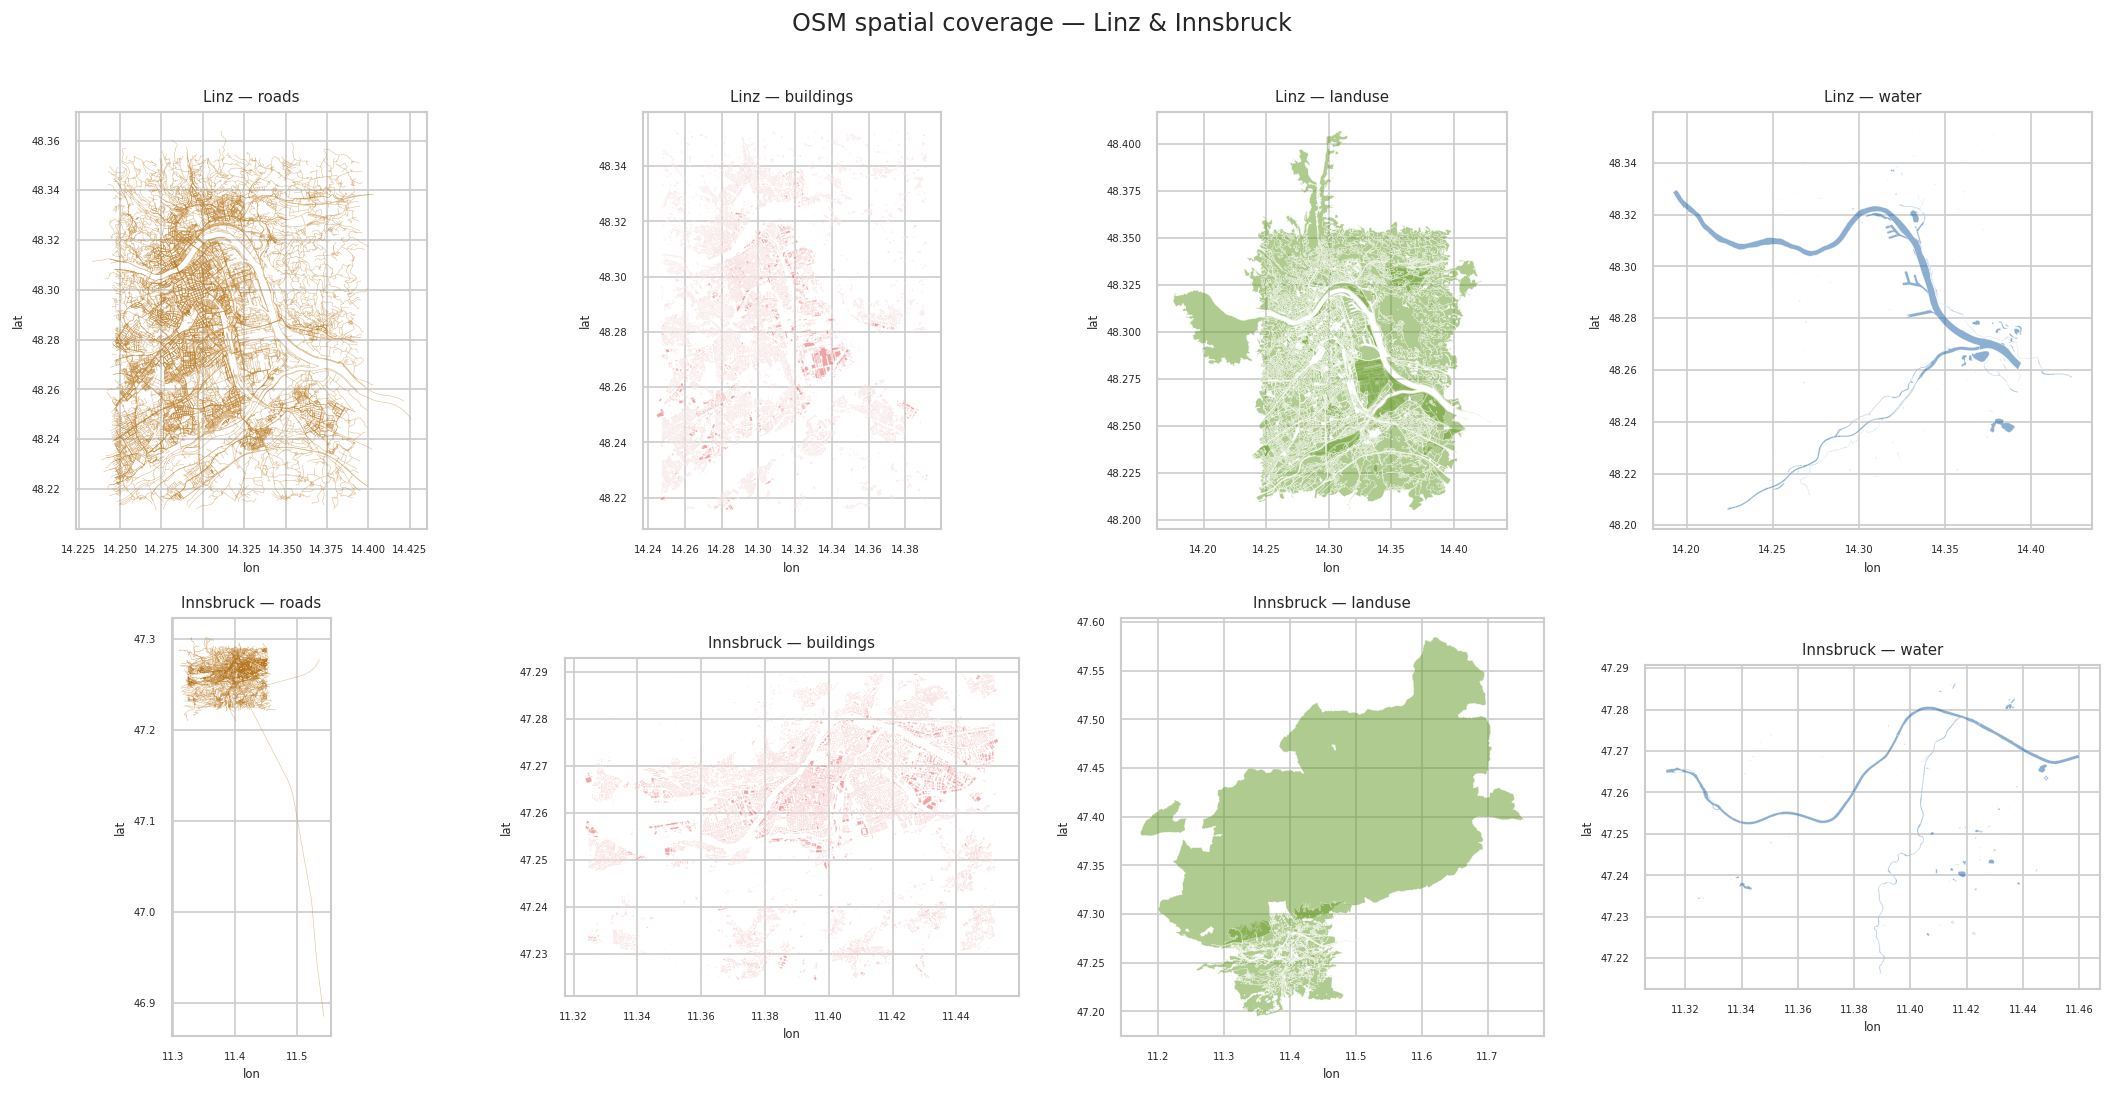
\includegraphics[width=\textwidth]{images/eda_p3_fig13.png}
\caption{Spatial coverage Linz and Innsbruck.}
\label{fig:geospatial-new}
\end{figure}


\begin{figure}[htbp]
\centering
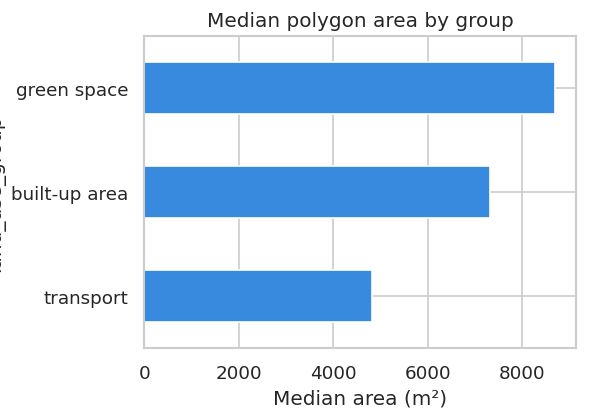
\includegraphics[width=0.72\textwidth]{images/eda_p3_fig14_b.png}
\caption{Median polygon area by group.}
\label{fig:combined-corpus-b}
\end{figure}

\newpage
\subsubsection{Sentinel-2: Innsbruck and Linz}

Sentinel-2 composites were successfully retrieved for both cities across three seasons.
Table~\ref{tab:ndvi-new} shows mean NDVI values per city and season.

\begin{table}[h]
\centering
\caption{Mean NDVI for Innsbruck and Linz by season (corrected TIFs, 2025 composites).}
\label{tab:ndvi-new}
\begin{tabular}{lrrrrr}
\hline
\textbf{City} & \textbf{Spring (Apr)} & \textbf{Summer (Aug)} & \textbf{Autumn (Nov)} &
\textbf{$\Delta$ Sp$\to$Su} & \textbf{$\Delta$ Su$\to$Au} \\
\hline
Linz       & 0.555 & 0.568 & 0.509 & $+0.013$ & $-0.059$ \\
Innsbruck  & 0.536 & 0.642 & 0.286 & $+0.106$ & $-0.356$ \\
\hline
\end{tabular}
\end{table}

Linz exhibits a stable, high NDVI across all three seasons, suggesting a predominantly
mixed-canopy character with dense urban green coverage consistent with an Austrian
mid-sized city.
Innsbruck shows a markedly different pattern: summer NDVI peaks at 0.642, higher than
any of the primary training cities in summer, while autumn NDVI falls sharply to~0.286,
a drop of $-0.356$ from summer.
This pronounced phenological signal reflects Innsbruck's Alpine geography: the city is
surrounded by deciduous valley-floor vegetation and steep forested slopes that lose
their canopy rapidly in October--November.
This steep gradient makes Innsbruck a particularly informative training example for the
temporal attention mechanism, which must learn to weight the less-informative autumn
timestep down relative to spring and summer.

Figure~\ref{fig:false-color-new} shows the false-color composites across all three seasons. Healthy vegetation appears bright red.
The strong seasonal change in Innsbruck is clearly visible in the autumn composite, where the valley vegetation and surrounding slopes substantially degreen.

\begin{figure}[h]
\centering
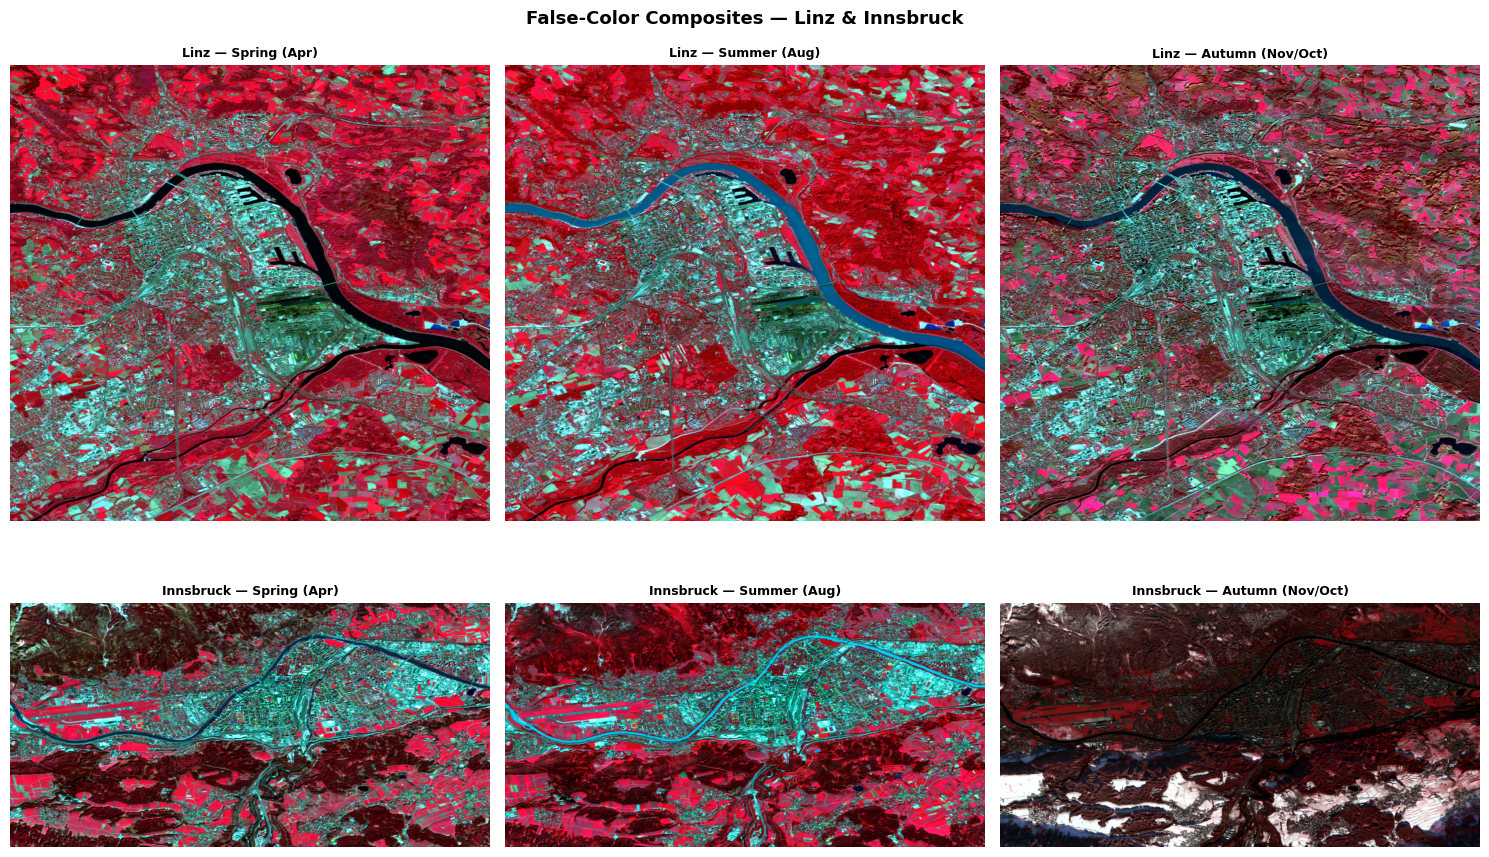
\includegraphics[width=\textwidth]{images/sent_p2_fig04.png}
\caption{False-color composites (NIR/Red/Green) for Innsbruck (top) and Linz
(bottom) }
\label{fig:false-color-new}
\end{figure}

All six Innsbruck and Linz TIFs passed data-quality checks with more than 95\% usable
pixels.
A single EVI artefact was found in the Innsbruck November file (0.76\% of pixels
out of bounds, mean value $-1.04 \times 10^{8}$, caused by near-zero denominators in
haze pixels over the Inn river).
This was resolved by recomputing EVI with a denominator guard and masking affected
pixels to NaN; corrected files were saved alongside the primary-city stack in
\texttt{data\_after\_eda/sentinel~data/}.

\subsection{Model Results}
On first sight the model overall achieves poor results with precision around 30% and recall around 40% and MAE of a bit higher than 1.1. Most of this can be attributed to the model having difficulties detecting single trees at a very low resolution where each pixel is 10m wide. Also, the imperfect ground truth with missing trees on private property makes it hard for the model to achieve good results. Other factors like trees being cut down during the year or small clouds which are difficult to detect for the model may also have an impact on model performance but are very negligible. 
\\
Better results can be seen when checking the actual predicted trees of the model manually, either by tediously checking for each tree on Google Earth or similar sites or by comparing the input image to the output image with the expected trees. So here are some representative examples both from Barcelona which was test data and from those parts of Vienna which were used for validation. 
\\
In those pictures we can see some very interesting phenomena. Firstly, that the model predicts a lot more trees than are in the ground truth which is a good thing, as we know that a lot of trees are not labeled. Furthermore, it also detects trees in areas where no trees are in the ground truth, so the model learns how a tree looks and can implement this knowledge also on wrongly labeled pixels. 

\begin{figure}[H] 
    \centering
    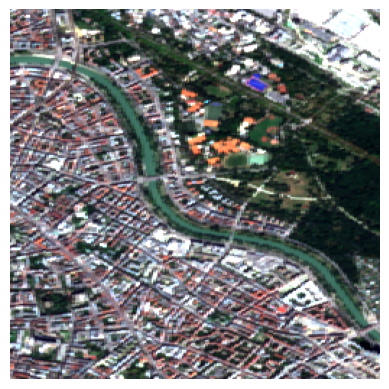
\includegraphics[width=\textwidth]{images/vie_img.png}
    \caption{RGB image of Vienna in August 2025}
\end{figure}
\begin{figure}[H] 
    \centering
    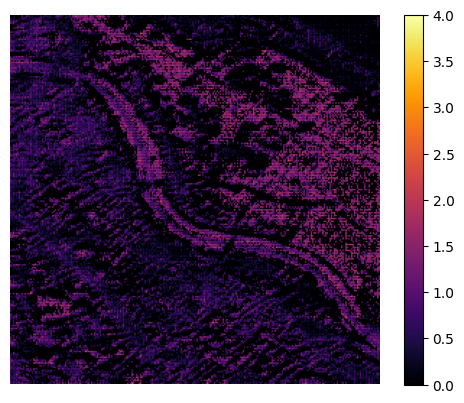
\includegraphics[width=\textwidth]{images/vie_pred.png}
    \caption{Model predictions for Vienna}
\end{figure}
\begin{figure}[H] 
    \centering
    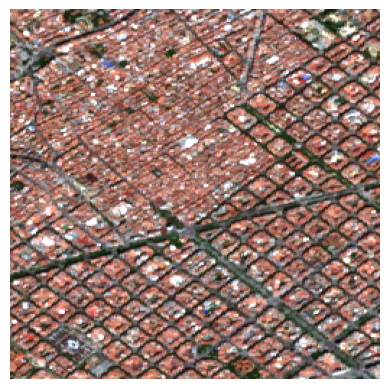
\includegraphics[width=\textwidth]{images/bar_img.png}
    \caption{RGB image of Barcelona in August 2025}
\end{figure}
\begin{figure}[H] 
    \centering
    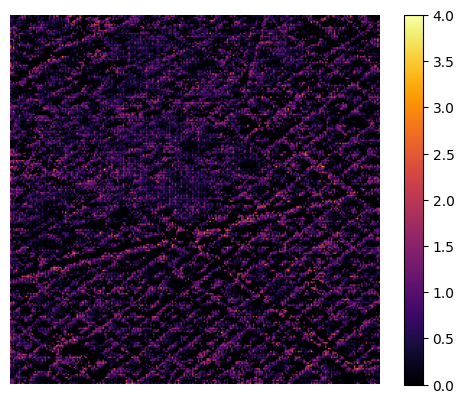
\includegraphics[width=\textwidth]{images/bar_pred.png}
    \caption{Model predictions for Barcelona}
\end{figure}
